\section{Information and Communication Technologies in Developing Countries}
Giving attention to \gls{ict}'s in the developing countries are both rewarding and useful. 
The potential impact \gls{ict}'s have in developing countries are much greater than in the industrialized countries. 
An innovative \gls{ict}'s step in the industrialized countries may lead to some improvement in productivity, but focusing our efforts in the developing countries has the potential of a much bigger impact.
The world problems of conflict, disease and resource depletion are first met by the poor. 
Although the more advanced economies of the world are not primary victims, it is beneficial to give these problems some attention.
These problems may someday reach the industrialized countries someday through terror, disease epidemics and migration. 
Also there is the added benefit of making the poor richer leads to the poor buying more products. Win-win.
In the 21st century, economic, social and political life are increasingly becoming more digital. 
This is also the case for the developing countries. 

The computers entered the developing countries in 1954. It started with Kolkata in India.
Initially computing was used in the public sectors for administrative tasks, but in the 1980's some saw \gls{ict}'s potential for economic growth in the private sector.
With the internet really catching on in the 1990's and politicians focusing on international development, much attention was given to \gls{ict}'s.
This gave rise to term \gls{ict4d}, popularized in literature.
As a result, many \gls{ict} initiatives took place in developing countries as a result of aid projects.
The most usual being tele-centers.
These were buildings housing computers giving people access to the world wide web.
The initiative had some problems succeeding, but brought with them important lessons that are still challenges we are facing today.
Sustainability, scalability and evaluation of systems in the developing countries are important topics to consider.
The systems of the past had a tendency to fail to deliver, have a limited reach and was generally talked about as better outcomes than it in reality was.
Today there is a internet penetration of $34.3\%$.
Looking forward, one of the main goal should be to give internet access to the remaining $65.7\%$ of the population.
In order to do this, we have to make \gls{ict} more available in developing countries.
Introducing \gls{ict}'s can done in three general different ways.
One could just set up an environment and make the users adapt to existing processes. 
Work with the users and continually innovate making locally appropriate solutions, or just introduce the technology and have the users innovate on their own. 
\cite{internet:stats}
\cite{icd4d:rh}
Looking at the literature on the topic of \gls{ict}'s in developing countries.
The success of \gls{is} projects are lower than those of the western countries like Europe and the \gls{usa}.
It is commonly dominated with themes like;
\begin{quotation}
Health information systems in South Africa: Braa
and Hedberg (2002) reported widespread partial
failure of high cost systems with little use of data.\cite{rh:isdc}
\end{quotation}

\begin{quotation}
IS in the Thai public sector: Kitiyadisai (2000)
reported “failure cases seem to be the norm in
Thailand at all governmental levels.”\cite{rh:isdc}
\end{quotation}

\begin{quotation}
Donor-funded IT projects in China: Baark and
Heeks (1999) reported that all were found to be
partial failures.\cite{rh:isdc}
\end{quotation}

\begin{quotation}
World Bank-funded IT projects in Africa: Moussa
and Schware (1992) reported almost all as partial—
often sustainability—failures.\cite{rh:isdc}
\end{quotation}

The evidence base are unfortunately not that strong due to lack of literature and evaluation.
The literature on \gls{ict} projects in developing countries are growing, but there are a tendency to focus on case studies, this paper included.
The lack of evaluation are often due to people who are performing these studies are coming up short with resources and capacity.
Like academics.
But from the literature there are some patterns seems to persist.

\begin{itemize}
\item Scarce resources
\item Little technology
\item Missing skills
\item \gls{is}-failure
\end{itemize}

In order to properly identify the different causes for failure we should try to define how something can be categorized as failure or success.

\subsection{Success and Failure of ISDC}
\begin{quotation}
Focus on case studies: The literature on IS in
DCs has grown, but it is a literature dominated by
case studies of individual IS projects. Taken alone,
these provide no basis for estimation of overall
failure/success rates.\cite{rh:isdc}
\end{quotation}
\label{successandfailure}
\begin{description}
\item[Total Failure] An initiative that never is implemented or abandoned immediately after implementation.
\item[Partial Failure] An initiative where major goals are unattained or where there are significant undesirable outcomes.
\item[Success] An initiative where major goals are attained for most stakeholders and there are no significant undesirable outcomes.
\end{description}

\begin{figure}
\centering
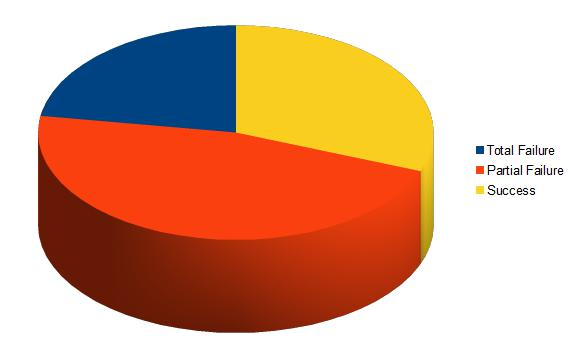
\includegraphics[width=\textwidth]{literature/img/failChart}
\caption{Diagram of average success and failures in \textbf{Industrialized Countries}}
\label{fig:failchart}
\end{figure}

Since there is a focus of case studies it is difficult to get an overall estimate for failure/success rates, but it generally points in one direction. High rates of \gls{is}-failure.


An overview of industrialized countries are presented in figure \ref{fig:failchart}.
In industrialized countries there is an estimate of $\frac{12}{60}$ to $\frac{15}{60}$ that falls into the category of total failure; something like $\frac{20}{60}$ to $\frac{36}{60}$ falls in the partial failure category; and lastly the $\frac{9}{60}$ to $\frac{28}{60}$ are successes.
For practical reasons like lack of technical and human infrastructure, developing countries should be performing worse than industrialized countries.
Failure can be viewed as something positive. 
Like in a learning process, but it cannot be overlooked that continually failing keeps the under developed countries on the wrong side of the digital divide. 

Borrowing terms from system transition, there are a higher risk of failure when moving to fast between source and target systems.
Fast being a revolutionary approach and slow an evolutionary.
Introducing \gls{ict} solutions from the industrialized countries would in fact become revolutionary seen from a developing countries perspective, even though they seem evolutionary from an industrialized perspective. 
The target systems are at very different stages.
Introducing an \gls{ict} system in developing countries therefore involves bigger risks.
\gls{ict} projects also are under a lot of pressure. Developing countries are trying to catch up with the industrialized countries. They have high opportunity costs and usually have over optimistic expectations.

\cite{rh:isdc}
\cite{ca:isdc}

\subsection{Pitfalls in introducing IS in Developing Countries}
The most common reasons for failure are related to scalability and sustainability.
\subsubsection{Scalability}
Scalability failure are usually caused of waning political support, technological complexity and the lack of human resource capacity. It is the problem of moving expertise and system to new locations with the lessons learned. By conceptualize the use of \gls{ict}'s one can make it easier to transfer \gls{ict}'s to other locations, making it scalable.
\cite{jbemss:noa}.
\subsubsection{Sustainability}
Common reasons for sustainability failure are by starvation of \gls{is} resources, loose political commitment and poor maintenance. 
Also there is a need to address the problem that arises when aid-funded projects stops being funded.
How does one maintain a project that is built on temporary donors?
One answer to this is by building on the locals capabilities and making projects that are socially embedded. The \gls{ict} project needs to be an integrated part of organizational practices, have   the required financial resources, knowledge resources and political commitment in order to succeed.
\cite{jbemss:noa}.  


\subsection{Discourses}
\label{subsec:discourses}

The pace and direction are mostly set by the advanced economic in the world.
The studies of \gls{ict} in developing countries are mostly set in Africa, Asia and Latin America.
These studies highlight new topics in the \gls{ict} literature including national culture, global politics, provision of \gls{ict} resources for a community.
By new topics there are also new approaches for introducing \gls{ict}'s, usually with the involvement of social sciences.
These three discourses generalizes these approaches;
\begin{description}
\item[\textit{Transfer and Diffusion Discourse}]
	The Transfer and Diffusion discourse assumes that \gls{is}-innovations in developing countries are achieved by transferring technology and organizational structure from more advanced countries. Much like, "if it works here, it should work there". In order to succeed the receiving part should try to emulate what is being done in the more developed countries. Of course \gls{is} these ideas of best practice are somewhat adapted to fit their new context, but the underlying assumption is that the transferred methods result in the same outcomes.
\item[\textit{Social Embeddednes Discourse}]
	This discourse assumes that \gls{is} innovation is about creating new techno-organizational structures given a local social context. The new structures are built on the already existing structures and are a locally socially constructed course of action. The problems are seen from a local perspective and hence the solutions has to be an integrated part.
\item[\textit{Transformative Discourse}]
	The last discourse is mostly concerned with creating possibilities for improvement of life conditions. It focuses on how \gls{is} can be used to facilitate deep socio-economic change.
	The social embeddednes discourse takes the local context into consideration, but the transformative takes it one step further and includes politics, economics and social conditions. 
\end{description}

The transformative discourse raises more explicitly the strategic issues in the development struggle.
A distinctive feature of \gls{is} research in developing countries is that it puts focus on e-governments, free and open software and the development of community resources intended to overcome the digital divide.
Diffusion and transformative development does not facilitate the already existing structures of the context the technology will be placed within.
The implementation of information systems from this perspective requires the environment and the people in it to adapt to the new technology.
This will in turn increase the risk of the information system being rejected by the users. On the other hand, the socially embedded path
will to some extent safeguard the underlying social structures by building upon what is already there. 
This might lead to unexpected results and be time consuming. Although, probably avoiding the sustainability pitfall.

\cite{ca:isdc}


\subsection{Networks of Action}
Networks of Action is a principle that sets out to remedy the sustainability failure of \gls{is}'s in developing countries. 
A common problem with \gls{is}-initiatives, then especially action research initiatives, is that the fail to persist over time.
Usually they fail to persist when researchers leave or donor funded projects stops. 
The basic principle is that the scale of the intervention will result in a more robust intervention. 
This changes most common perspective of seeing scale and sustainability as two different problems. 
Rather it views scale as a prerequisite in order to achieve sustainability.
This argues for \gls{is} initiators to form alliances with surrounding network in order to succeed. 
Establishing networks creates opportunities for sharing experiences, knowledge  and technology between different actors. 

Building networks running on the same concept will make the ICT initiative more sustainable. 

User participation is another tool one can use in order to make ICT initiative more sustainable.
When the concept is accepted and made by the users they understand how and why it works and are more likely to accept it.

\cite{jbemss:noa}








